\documentclass[border=10pt]{standalone}
\usepackage[svgnames]{xcolor}
\usepackage{amsmath}
\usepackage{pgfplots}
\pgfplotsset{compat=newest}
\usepackage[sfdefault]{FiraSans}
\usepackage{FiraMono}
\renewcommand*\familydefault{\sfdefault}
\begin{document}
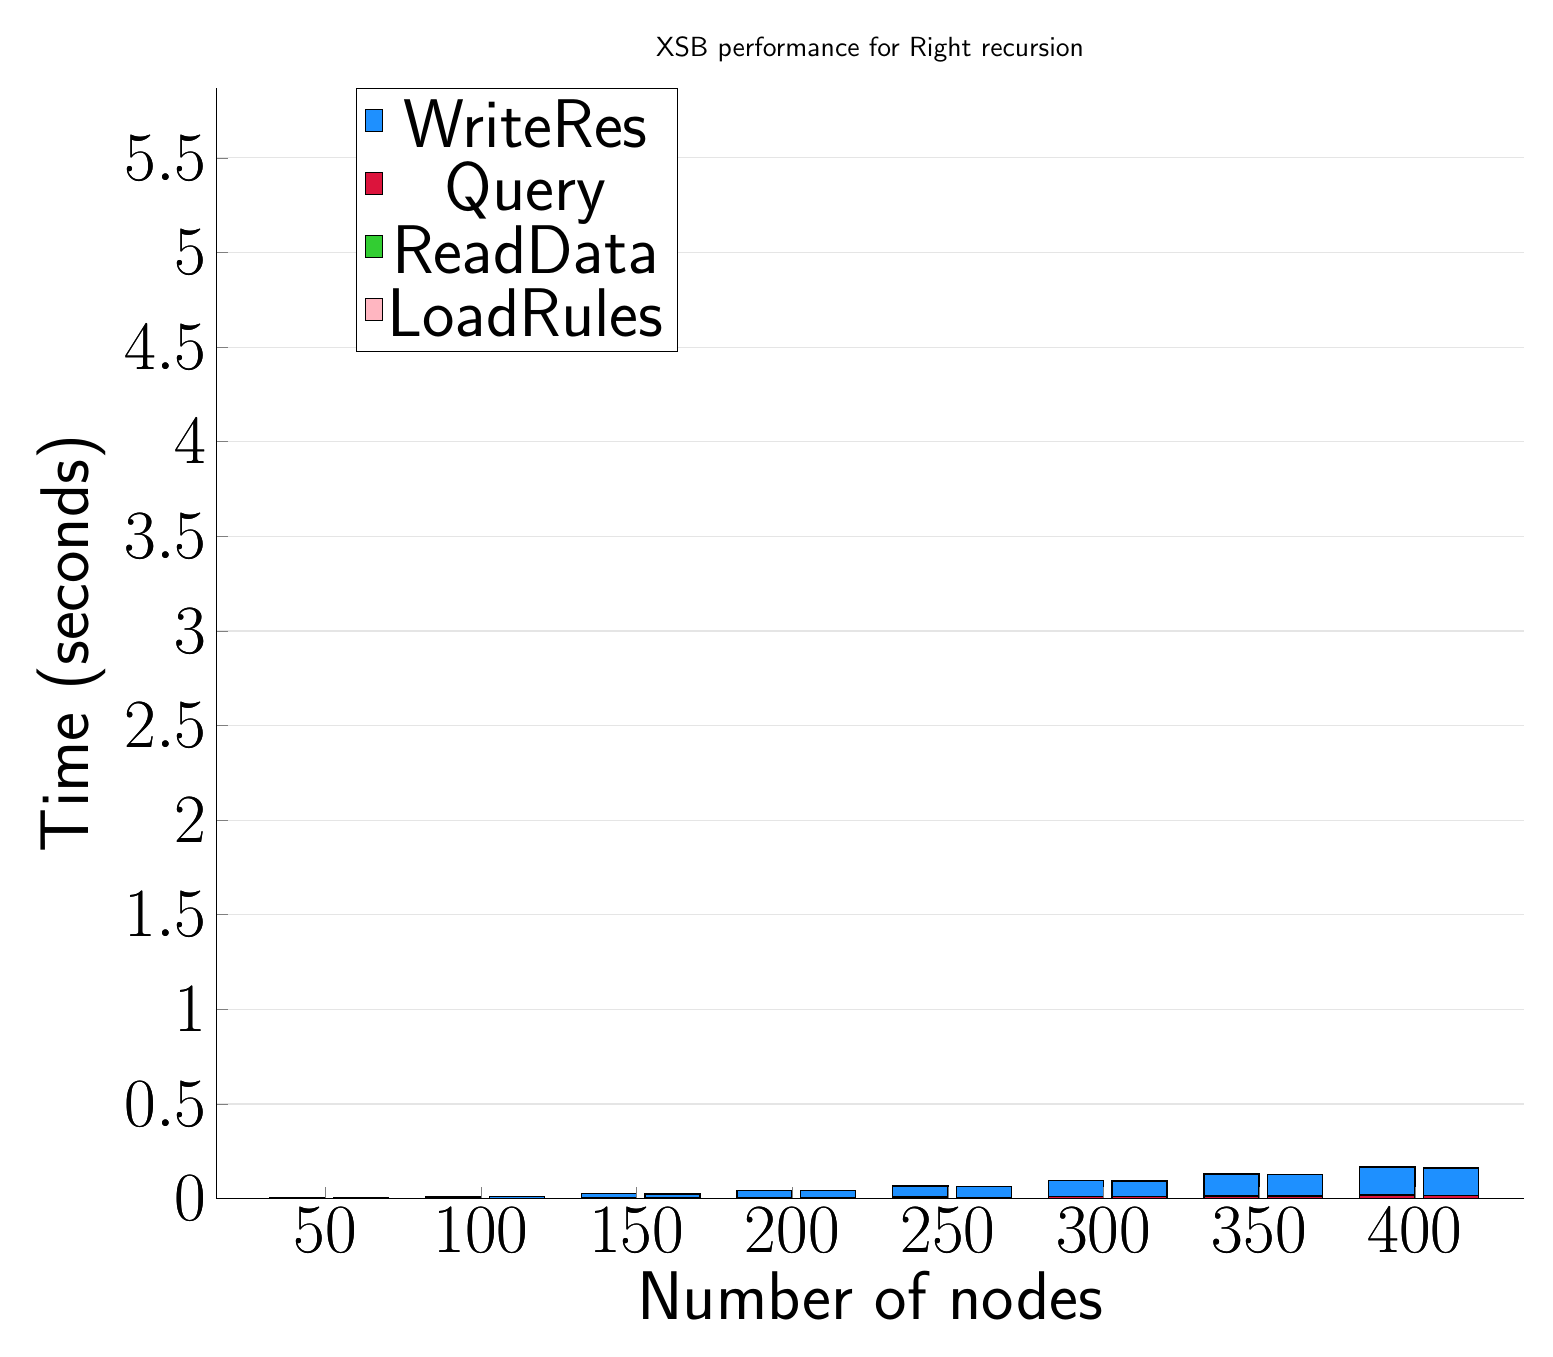
\begin{tikzpicture}
	\begin{axis}[
			ybar stacked,
			title={XSB performance for Right recursion},
			bar shift=-10pt,
			width=1.5\textwidth,
			bar width=0.7cm,
			ymajorgrids, tick align=inside,
			major grid style={draw=gray!20},
			xtick=data,
			ymin=0, ymax=5.870271515846253,
			axis x line*=bottom,
			axis y line*=left,
			enlarge x limits=0.1,
			legend style={
					at={(0.23, 1)},
					anchor=north,
					legend columns=1,
					font=\Huge,
				},
			ylabel={Time (seconds)},
			xlabel={Number of nodes},
			label style={font=\Huge},
			tick label style={font=\Huge},
		]
		\addlegendimage{fill=DodgerBlue, draw=black, line width=0.2pt}
		\addlegendentry{WriteRes}
		\addlegendimage{fill=Crimson, draw=black, line width=0.2pt}
		\addlegendentry{Query}
		\addlegendimage{fill=LimeGreen, draw=black, line width=0.2pt}
		\addlegendentry{ReadData}
		\addlegendimage{fill=LightPink, draw=black, line width=0.2pt}
		\addlegendentry{LoadRules}
		\addplot +[fill=LightPink, draw=black, line width=0.5pt] coordinates {
				(50, 0.001119852066040039)
				(100, 0.001030349731445313)
				(150, 0.0010356187820434568)
				(200, 0.001099085807800294)
				(250, 0.001052236557006835)
				(300, 0.001092910766601563)
				(350, 0.001101636886596679)
				(400, 0.001068377494812013)
			};
		\addplot +[fill=LimeGreen, draw=black, line width=0.5pt] coordinates {
				(50, 0.0003966331481933593)
				(100, 0.00043888092041015635)
				(150, 0.00047700405120849616)
				(200, 0.0005544662475585936)
				(250, 0.0005922079086303711)
				(300, 0.0006494998931884765)
				(350, 0.0006862878799438477)
				(400, 0.0007074117660522461)
			};
		\addplot +[fill=Crimson, draw=black, line width=0.5pt] coordinates {
				(50, 0.0002847671508789064)
				(100, 0.001041722297668457)
				(150, 0.002311301231384277)
				(200, 0.004150962829589844)
				(250, 0.006200170516967774)
				(300, 0.009373831748962402)
				(350, 0.012830305099487311)
				(400, 0.016482996940612803)
			};
		\addplot +[fill=DodgerBlue, draw=black, line width=0.5pt] coordinates {
				(50, 0.0026171684265136725)
				(100, 0.009773993492126473)
				(150, 0.021636819839477545)
				(200, 0.03774075508117676)
				(250, 0.059625267982482924)
				(300, 0.08413536548614502)
				(350, 0.1148846387863159)
				(400, 0.1484114646911621)
			};
	\end{axis}
	\begin{axis}[
			ybar stacked,
			bar shift=13pt,
			width=1.5\textwidth,
			bar width=0.7cm,
			ymajorgrids, tick align=inside,
			major grid style={draw=none},
			xtick=data,
			ymin=0, ymax=5.870271515846253,
			axis x line*=none,
			axis y line*=none,
			enlarge x limits=0.1,
			label style={font=\Huge},
			tick label style={font=\Huge},
		]
		\addplot +[fill=LightPink, draw=black, line width=0.5pt] coordinates {
				(50, 0.0006333)
				(100, 0.0005995)
				(150, 0.0006054)
				(200, 0.0006274999999999999)
				(250, 0.0006001000000000001)
				(300, 0.0006181999999999998)
				(350, 0.0006144999999999998)
				(400, 0.0006131000000000004)
			};
		\addplot +[fill=LimeGreen, draw=black, line width=0.5pt] coordinates {
				(50, 0.0001802999999999996)
				(100, 0.0002196999999999999)
				(150, 0.00026230000000000014)
				(200, 0.0003135999999999998)
				(250, 0.00035130000000000024)
				(300, 0.00039990000000000007)
				(350, 0.00044700000000000046)
				(400, 0.0004748999999999993)
			};
		\addplot +[fill=Crimson, draw=black, line width=0.5pt] coordinates {
				(50, 0.0002576999999999999)
				(100, 0.0009696999999999998)
				(150, 0.0021565)
				(200, 0.0038309999999999998)
				(250, 0.005784600000000001)
				(300, 0.0087443)
				(350, 0.0119166)
				(400, 0.015354399999999999)
			};
		\addplot +[fill=DodgerBlue, draw=black, line width=0.5pt] coordinates {
				(50, 0.0023225000000000003)
				(100, 0.009300600000000001)
				(150, 0.0209035)
				(200, 0.036817)
				(250, 0.0573877)
				(300, 0.08264429999999999)
				(350, 0.1128278)
				(400, 0.1456286)
			};
	\end{axis}
\end{tikzpicture}

\end{document}
